\documentclass{article} % For LaTeX2e
\usepackage{nips13submit_e,times}
\usepackage{hyperref}
\usepackage{url}
\usepackage{todonotes}
\usepackage{paralist}
\usepackage{bm}
\usepackage{amsmath}
\usepackage{float}
\usepackage[bottom]{footmisc}
%\documentstyle[nips13submit_09,times,art10]{article} % For LaTeX 2.09


\title{Customer Feedback Topic Modelling Using Online Latent Dirichlet Allocation}


\author{
Yuhou Zhou\\
Department of Computer Science \& Electrical Engineering\\
Jacobs University Bremen\\
Bremen, Germany\\
Corporate Information Management\\
CEWE Stiftung \& Co. KGaA\\
Oldenburg, Germany\\
\texttt{yu.zhou@jacobs-university.de}\\
\texttt{yuhou.zhou@cewe.de}\\
}

\newcommand{\fix}{\marginpar{FIX}}
\newcommand{\new}{\marginpar{NEW}}

\nipsfinalcopy % Uncomment for camera-ready version

\setlength {\marginparwidth }{2cm}
\begin{document}
    \raggedbottom
    \maketitle

    \begin{abstract}
        % Two line spaces precede the abstract.
        % The abstract must be limited to one paragraph.
        I develope a topic modelling system\footnote{Available on \textit{gitlab.com/yuhouzhou/cftm}} for extracting topics from customer feedback. The system includes three parts which are preprocessing, modelling, and visualization. Apache PySpark helps to read large volume data, and Python spaCy is used to run preprocessing pipeline. Online Latent Dirichlet Allocation is the selected topic model, and the system uses Gensim implementation. Topic coherence serves as the evaluation metric for choosing the optimal topic number. LDAvis presents topic modelling results interactively and shows the topic distribution over two principal components. This project can serve as a base for further generalizing to extract topics from different data sources.
    \end{abstract}

    \section{Introduction}

    Customer feedback is information provided by clients about their general experience
    with a product or a service. At CEWE, one method to collect such feedback is asking
    customers to complete online survey.

    By collecting customer feedback, the extracted information can act as a guide to
    improve products. Feedback gives the company the clue of customers' general experience
    and the satisfaction rate. Except the description provided by sellers, the publicly
    posted feedback is useful information to other consumers, imparting them an overview
    how the product really is. This information also helps managers to make correct business
    decisions.

    The current way of processing user feedback requires that working staff reads the
    feedback and later extracts topics. This process can be costly and inefficient,
    because of manual intervention. At one time, people can only process a small batch of
    text from a recent period. Thus, the information, which concerning long lasting but
    less frequently appeared issues, may lost.

    Latent Dirichlet Allocation (LDA) can automate this topic extraction process. LDA is a generative probabilistic model for discrete data, and it is especially popular in the field of topic modelling.
    In this project, I automate the topic extraction process utilizing Online Latent Dirichlet Allocation with the optimal number of topics found by topic coherence.

    \section{Related Work}
    \label{gen_inst}

    Discovering “topics” from a collection of documents has been a long-standing problem
    in natural language understanding. Latent Semantic Analysis (LSA) acts as the base of
    recent topic models \cite{deerwester_indexing_1990}. Hofmann proposed Probabilistic Latent Semantic Indexing (pLSA) \cite{hofmann_probabilistic_2017}, bringing topic models from deterministic to probabilistic. Blei et al. (2003) described Latent Dirichlet Allocation (LDA) which is a Bayesian alternative to pLSA \cite{blei_latent_2003}. LDA makes use of word co-occurrence information in documents, to generate document-topic distribution. Hoffman et al. (2010) developed an online variational Bayes algorithm for LDA \cite{hoffman_online_2010}. This online version of LDA was demonstrated that it has advantages over batch LDA in terms of model accuracy and the modelling time.
    However, the lack of word co-occurrence in short texts prevents LDA yielding satisfying
    results \cite{li_topic_2016}. Such short texts are news headlines, tweets, user feedback, questions and answers, and so on. One strategy to overcome this data sparsity problem is to concatenate a set of short texts according to available metadata \cite{weng_twitterrank:_2010, hong_empirical_2010, mehrotra_improving_2013}. For example, aggregating texts by timestamps, locations or users.

    Perplexity was used to evaluate the accuracy of topic models \cite{wallach_evaluation_2009}. However, Chang et al (2009) found that perplexity does not always correlated with the interpretability of topics \cite{chang_reading_2009}. Topic coherence c\textunderscore{}uci was first proposed by Newman et al.(2010)\cite{newman_automatic_nodate}, by using pairwise pointwise mutual information (PMI) between the topic words. c\textunderscore{}uci was proven highly correlated with human judgment. Röder et al. (2015) proposed topic coherence c\textunderscore{}v which was identified that it outperformed other topic coherence \cite{roder_exploring_2015}.

    \section{Online Latent Dirichlet Allocation}
    Latent Dirichlet Allocation is an unsupervised machine learning model \cite{blei_latent_2003}. It identifies latent topics in corpus. Each document in the corpus is represented as probability distribution over some other topics. All the topics are represented as a probability distribution over some words.

    Theoretically, a document $\bm{w}$ in the corpus $D$ is associated with a multinomial distribution over $T$ topics; $T$ is the predefined number of topics, and document is denoted by $\bm{w} = (w_1, w_2, ..., w_N)$ where $w_n$ is the $n$th word in the sequence. The multinomial distribution is denoted as $\theta$. One topic is similarly associated with a multinomial distribution $\phi$ over words $w_n$.

    $\theta$ and $\phi$ whose hyper-parameters are $\alpha$ and $\beta$ respectively have Dirichlet prior. For every word in one document $\bm{w}$, a topic $z$ is sampled consequently. This generative process is repeated $N$ times, where $N$ is the number of words in the document \cite{hong_empirical_2010}.

    A k-dimensional Dirichlet Random variable has the following probability density:
    \begin{align}
        p(\theta|\alpha) = \frac{\Gamma(\sum_{i=1}^{k} \alpha_i)}{\Pi_{i=1}^{k}\Gamma(\alpha_i)}\theta_{1}^{\alpha_{1}-1}\dots\theta_{k}^{\alpha_{k}-1}
    \end{align}
    where $\Gamma(x)$ is the Gamma function.
    The probability of a corpus:
    \begin{align}
        p(D|\alpha, \beta) = \displaystyle \prod_{d=1}^{M}\int p(\theta_{d}|\alpha) \left( \displaystyle  \prod_{n=1}^{N_d}\sum_{z_{dn}}p(z_{dn}|\theta)p(w_{dn}|z_{dn}, \beta) \right)d\theta_d
    \end{align}
    The probabilistic graphical model representation of LDA is in Figure 1. As shown in the Figure 1, LDA consists of three layers. The parameters $\alpha$ and $\beta$ are one the level of corpus. $\theta_{d}$ are variables on the level of document. $z_{dn}$ and $w_{dn}$ are variables on the level of word.

    However batch LDA still requires to feed the entire corpus into each iteration when the model is being trained. Thus, in some circumstance LDA does not perform well, such as when the datasets are large, or when new data comes in stream to the training process \cite{hoffman_online_2010}.
    \begin{figure}[H]
        \graphicspath{ {images/} }
        \begin{center}
            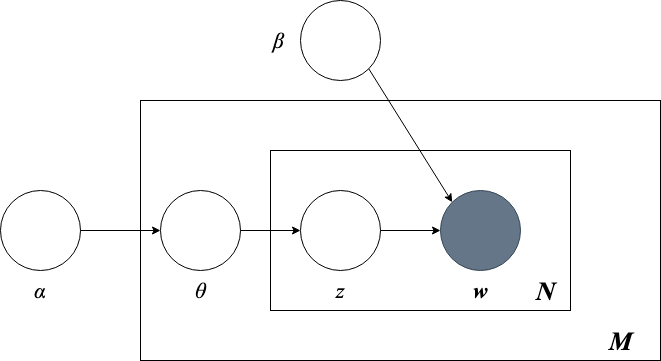
\includegraphics[scale=0.4]{LDA.png}
        \end{center}
        \caption{Graphical model representation of LDA}
    \end{figure}
    \todo[inline]{online version}

    \section{Topic Coherence}
    By combining elementary components, Röder et al proposed the topic coherence c\textunderscore{}v, which was proved that it outperforms other topic coherence \cite{roder_exploring_2015}.

    \section{Visualization}
    In 2014, Sievert et al. presented a web-based visualization for Latent Dirichlet Allocation \cite{sievert_ldavis:_2014}

    % \section{Approach}
    % \label{headings}

    % Data preparation is performed to filter information and concatenate entries of feedback according to their metadata. Afterwards a LDA model will be trained on previous customer feedback. Topic coherence will be picked to measure the function of the model.

    % The used tools are Python spaCy, Apache Spark and Gensim. Spacy also supports German and is highly optimized. It has very good interfaces with other machine learning libraries, such as TensorFlow, scikit-learn. Gensim is a python library which is highly efficient and scalable towards topic and semantic modelling.

    % Two obstacles are about to be solved. The feedback is written in German is one of the difficulties. Nowadays, many natural language processing libraries have poor support to German language. Either they cannot train models based on German, or they only provide limited features to German. The other difficulty is the variation of text is dramatic and unpredictable. This is reflected on two aspects. First, the quality of the feedback is varying. Some feedback contains totally useless information, such as "Nein", the copy of the survey email. The length of the feedback varies from one word to a long text containing hundreds of words. Second, the content of new feedback is unforeseeable. It may include new products, new services, etc.

    % For model deployment, the model will be retrained based on a time period. Outdated observations will be removed, and new observations will be included into the training process. This process can be scheduled using an orchestrator tool, such as Apache Airflow.

    \section{Data File}
    The original data files used for this project are two parquet files of the overall size 1.47 GB. The parquet file in customer\textunderscore{}feedbacks/ contains 101 columns, and the one in customer\textunderscore{}feedbacks\textunderscore{}cat/ contains 7 columns. The content of customer feedback is stored in the column ANTWORT\textunderscore{}WERT, There are 1,917,490 feedbacks including duplicates since 14/04/2012.The sentiment of the feedback is stored in the column STIMMUNG.

    \section{System Architecture and Usage}
    Under the project root directory, there are cftm/ directory, environment.yml file and README.md file.

    environment.yml files specifies the environment dependencies of the system. We can use conda to recreate the system environment. README.md provide brief introduction of the system.

    The source code of the system is under cftm/cftm/ directory. It contains three python files which are pipeline.py, cftm\textunderscore{}parser.py, preprocessing.py and one yml file, path.yml file.

    pipeline.py is the entry of the system, passing arguments to this file in order to control the behavior of the system. cftm\textunderscore{}parser.py and preprocessing.py contains modules used by pipeline. cftm\textunderscore{}parser.py extracts specified data from data source file; preprocessing.py executes standard nlp preprocessing operations, eventually converting texts to the object which Gensim requires. path.yml file contains all the paths to store system output.

    \subsection{cftm\textunderscore{}parser.py}
    cftm\textunderscore{}parser.py contains one method parquet\textunderscore{}transform() to transform data in parquet files to the data format for preprocessing and modelling.

    \underline{\textit{parquet\textunderscore{}transform(path1, path2, n=-1)}}

    \textbf{parameters: }
    \begin{compactitem}
        \item path1 (str) - the path of the first parquet file
        \item path2 (str) - the path of the second parquet file
        \item n (int, optional) - the number of observations to be transformed. When the passed integer is smaller than 0, all observations from data source will be transformed.
    \end{compactitem}

    \textbf{returns:}
    \begin{compactitem}
        \item \textit{pandas.dataframe} - include the data frame with desired columns and the specified number of observations
    \end{compactitem}


    cftm\textunderscore{}parser makes use of Apache Spark, and Spark SQL to import data from parqurt file. Since the size of the parquet files are in the level of gigabytes, directly using method \textit{pandas.read\textunderscore{}parquet()} to extract pandas data frame requires large volume of memory. This is sometimes unrealistic when only a personal computer is available for running the system.

    An alternative way to import the data is using \textit{spark.read.parquet()}. Instead of fitting all the data to memory, Spark's operators spill data to disk, which make it possible to run over any size of data. \textit{spark.read.parquet()} reads a parquet file from a specified path and return a \textit{spark.data frame} object. Writing queries by Spark SQL makes the data manipulation the same as the process over relational database. After the query the size of the data drops significantly. Sequentially, duplicated observations are dropped and \textit{spark.dateframe} is transformed to \textit{pandas.data frame} for preprocessing procedures.

    \subsection{preprocessing.py}
    \textit{preprocessing.py} utilizes python spaCy to run the standard text preprocessing pipeline, which includes tokenization, lemmatization, lowercasing, striping white spaces, and removing stopwords and punctuations. A token is the name for a sequence of characters that we want to treat as a group, i.e. word, punctuation symbol, white space, etc. Tokenization means to convert a text to a collection of tokens. Lemmatization assigns the base forms of words. For example, assign "run" to "running", "ran", or "be" to "is", "am", "were", etc. Stopwords are the words which appear with high-frequency, such as "also", "the", "to", etc. They too ubiquitously exist in texts, and therefore contain little information about the text. Stopwords and punctuations are removed to only keep words which are distinct.

    spaCy\footnote{Available on \textit{github.com/explosion/spaCy}} is a Python/Cython natural language processing package which currently offers fastest syntactic parser in the word. Choi et al. (2015) conducted an evaluation research proved the outstanding performance of spaCy \cite{choi_it_2015}. The high speed of spaCy makes it especially suitable to processing large volume of text data.

    Four methods are in this script. \textit{text\textunderscore{}preproc\textunderscore{}maker()}, \textit{text\textunderscore{}aggregation()}, \textit{gensim\textunderscore{}prep()}, and \textit{preprocessor()}.

    \underline{\textit{text\textunderscore{}preproc\textunderscore{}maker(stopwords, language='de')}}

    A currying function which returns a new function \textit{text\textunderscore{}preproc(sentence)} to run the text preprocessing pipeline ,including tokenization, emmatization, lowercasing, striping white spaces, and removing stopwords and punctuations, for the specified language.

    \textbf{parameters: }
    \begin{compactitem}
        \item stopwords (list of str) - a list of stopwords
        \item language (str, optional) - the possible inputs are the languages which spaCy supports, such as 'de', 'en', etc. Before use the specified language, first install the spaCy required language, using command \textit{pip install spacy \&\& python -m spacy download en}, here 'en' can be replaced with the language you would like to install.
    \end{compactitem}

    \textbf{returns:}
    \begin{compactitem}
        \item \textit{text\textunderscore{}preproc object} - a function takes sentences as the parameter, containing the pipeline of preprocessing.
    \end{compactitem}

    \underline{\textit{text\textunderscore{}aggregator(df\textunderscore{}pd, metadata='DATE', min\textunderscore{}len=-1)}}

    \textbf{parameters: }
    \begin{compactitem}
        \item df\textunderscore{}pd (pandas.dataframe) - a Pandas data frame containing text data and metadata.
        \item metadata (str, optional) - the column name of the metadata which is used to aggregate texts. Legal options are 'DATE' and 'SENTIMENT'.
        \item min\textunderscore{}len (int, optional) - when the metadata is 'DATE', this argument decides the minimal length of the aggregated text. The default is -1, which means no aggregation, but using the original texts.
    \end{compactitem}

    \textbf{returns:}
    \begin{compactitem}
        \item \textit{list of lists of str} - the text data after aggregation.
    \end{compactitem}

    \underline{\textit{gensim\textunderscore{}prep(texts)}}

    This method converts list of lists string to gensim dictionary and corpus objects.
    \textbf{parameters: }
    \begin{compactitem}
        \item texts (list of lists of str) - text data.
    \end{compactitem}

    \textbf{returns:}
    \begin{compactitem}
        \item \textit{list of lists of str} - the text data.
        \item \textit{gensim.corpora.dictionary.Dictionary} - A mapping between words and their integer ids.
        \item \textit{list of lists of (int, int)} - Bag of words representation of the documents.
    \end{compactitem}

    \underline{\textit{preprocessor(df\textunderscore{}pd, stopwords, language='de', text='TEXT', metadata=None, min\textunderscore{}len=-1)}}

    This method wraps up preproc, text aggregator, and gensim\textunderscore{}prep to compose a full preprocessing pipeline. It returns text data, gensim dictionary, and gensim bag of words corpus. See the information of the arguments above.

    \subsection{pipeline.py}
    pipeline.py is the entry of the system. It consists of three parts preprocessing, modelling, and visualization. Preprocessing part uses the function \textit{preprocessor()} in preprocessing.py. For modelling, gensim implemented Online LDA is used. pyLDAvis module takes the training results from Online LDA, and produce a html file which supports interactive visualization.

    \subsubsection{Arguments}
    This program takes 9 arguments. \textit{--pipeline} is a positional argument, and others are optional arguments.

    \textit{--pipeline} is a positional parameter, requiring 3 integer numbers, which switches preprocessing, modelling, and visualization respectively. If one of the numbers is 0, the corresponding function is turned off. If it is none 0, the corresponding function is turned on. For example, if the parameter is \textit{1 1 1}, then the pipeline will be preprocessing, modelling, and visualization. If the parameter is \textit{0 1 1}, then the pipeline will only have the procedures of modelling and visualization, when the training data is read from a pickle file, which is either got from a archive or is copied to the required path. The parameter \textit{0 0 1} has the same logic. \textit{1 0 0} and \textit{1 1 0} also are the legal combinations. Designing the system in this way makes the pipeline flexible and fault tolerant. Since the data volume is big, user can choose which part of the pipeline he would like to run to avoid repeated work. Every part of the pipeline produces a pickle file to archive the outcome, so even if the program is stopped during a run, the results are saved and can be continued next run.

    \textit{--path\textunderscore{}file} or \textit{-p} is an optional parameter, requiring a str value. The default value is \textit{./path.yml}. It accepts a path of the yml file in which all output paths are indicated. The yml file uses a dictionary to store paths, and the keys are parquet\textunderscore{}path1,
    parquet\textunderscore{}path2,
    archive\textunderscore{}fore\textunderscore{}path,
    data\textunderscore{}path,
    model\textunderscore{}path,
    pic\textunderscore{}path,
    html\textunderscore{}path,
    log\textunderscore{}path.

    \textit{--observation\textunderscore{}n} or \textit{-o} indicates the number of observations used in the program, requiring an integer. The default value is -1, which means use all observations.

    \textit{--agg\textunderscore{}metadata} or \textit{-m} indicates the metadata which is used during the aggregation session. The default value is 'DATE', and the other legal value is 'SENTIMENT'.

    \textit{--agg\textunderscore{}length} or \textit{-l} indicates the minimal length of every document after an aggregation session, if the metadata 'DATE' is used. It requires an integer number, and the default value is -1, which means the aggregation is aborted.

    \textit{--topic\textunderscore{}range} or \textit{-r} indicates the topic range during the modelling session. It requires 3 integer numbers, meaning the minimal number of topics, the maximal number of topics, and the step. The default value is \textit{1 10 1}, so the modelling session will generate 10 LDA models with topic numbers from 1 topic to 10 topics.

    \textit{--chunksize} or \textit{-c} is an hyperparameter to Online LDA model. Online LDA algorithm update the model every chunksize. For example, if a corpus has 10000 documents, and the chunksize is set to 1000, then Online LDA will update the model 10 time through one complete pass of the corpus. The default value is 2000.

    \textit{--iteration} or \textit{-i} indicates the number of iterations during optimization, requiring an integer number. The number of iterations should high enough to make the model converge. However, fewer iterations make the modelling time shorter. The default value is 50.

    \textit{--seed} or \textit{-s} indicates the seed passed to LDA model, make the whole process replicable. The default value is 1.

    An example command can be \textit{python pipline.py 1 1 1 -p ./path.yml -o 40000 -m DATE -l 15 -r 10 50 5 -c 800 -i 400 -s 2},
    which means: run the complete pipeline (preprocessing, modelling, and visualization). In preprocessing, 40000 observations are included, and the
    system uses 'DATE' column as metadata to aggregate documents. After aggregation, every document has minimun length of 15 tokens. In modelling session,
    LDA models with topic numbers 10, 15, 20, ... , 50 are generated. 800 obeservations as a chunk is used for training, in this case, one full pass of
    corpus will update models $40000 / 800 = 50$ times. There are maximun 400 iterations through the corpus when inferring the topic distribution of the corpus.
    All the output files, such as processed training data, log files, lda models, topic coherence models, visualizations, etc, are saved in the paths
    specified in \textit{./path.yml}. The seed is set as 2.

    For every run of the program, parameters are saved in \textit{commandline\textunderscore{}args.yaml} file in the output folder and archive folders.

    \subsubsection{Modelling}
    gensim\footnote{Available on github.com/RaRe-Technologies/gensim} is an open-source library for unsupervised topic modelling and natural language processing. This software framework was proposed by {\v R}eh{\r u}{\v r}ek in 2010, featuring with its clarity, efficiency and scalability \cite{rehurek_lrec}. gensim supports parallel computing and is scalable through a cluster, which accelerate training process significantly. For this customer feedback topic extraction system, gensim Online LDA model is chosen.

If in one program run, the preprocessing stage is turned on. The processed data will be used in the model training session. If not, the training data
    will be read from previous pickled training data.

    The modelling session generates LDA models with number of topics passed to \textit{--topic\_range} or {-r} argument. For every model, its topic coherence is also
    generated. In this project, topic coherence \textit{c_v} is used, because it often outperforms other topic coherence \cite{}. After one model is trained and its topic
    coherence is evaluated, it will be dumped as \textit{.pickle} file. This is a full iteration of modelling, and next iteration the LDA model is
    passed with a topic number which is \textit{step-size} higher. In the end of every modelling iteration, the model and its topic coherence will be added
    to previous \textit{.pickle} file.

    \subsubsection{Visualization}
Visualization includes two parts. The first part is generating scatterplot, topic coherence of the model \textit{c\_n} against topic numbers. The higher the score of topic coherence
    often means better interpretability of the topics. The topic number with the highest topic coherence is marked red on the scatterplot. The second
    part is visualize the topics of the model with the highest topic coherence score, using python package pyLDAvis. The html file is dumped.

    \section{Results}
    % Example pictures
    % Comparing with concatenation and without concatenation
    \begin{figure}[H]
        \graphicspath{ {images/} }
        \begin{center}
            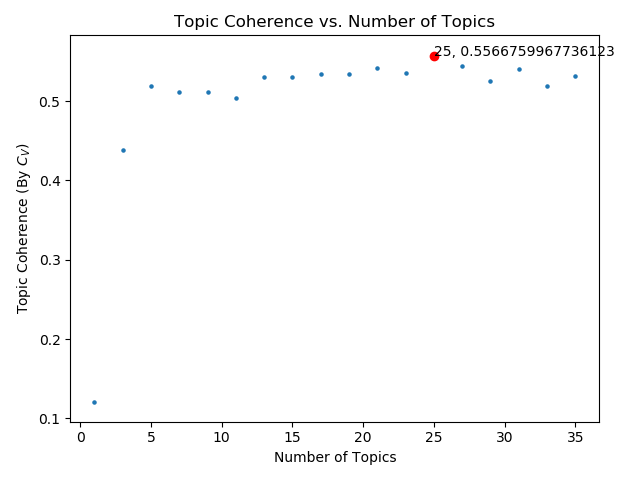
\includegraphics[scale=0.8]{coherence.png}
        \end{center}
        \caption{Topic Coherence vs. Number of Topics}
    \end{figure}

    \begin{figure}[H]
        \graphicspath{ {images/} }
        \begin{center}
            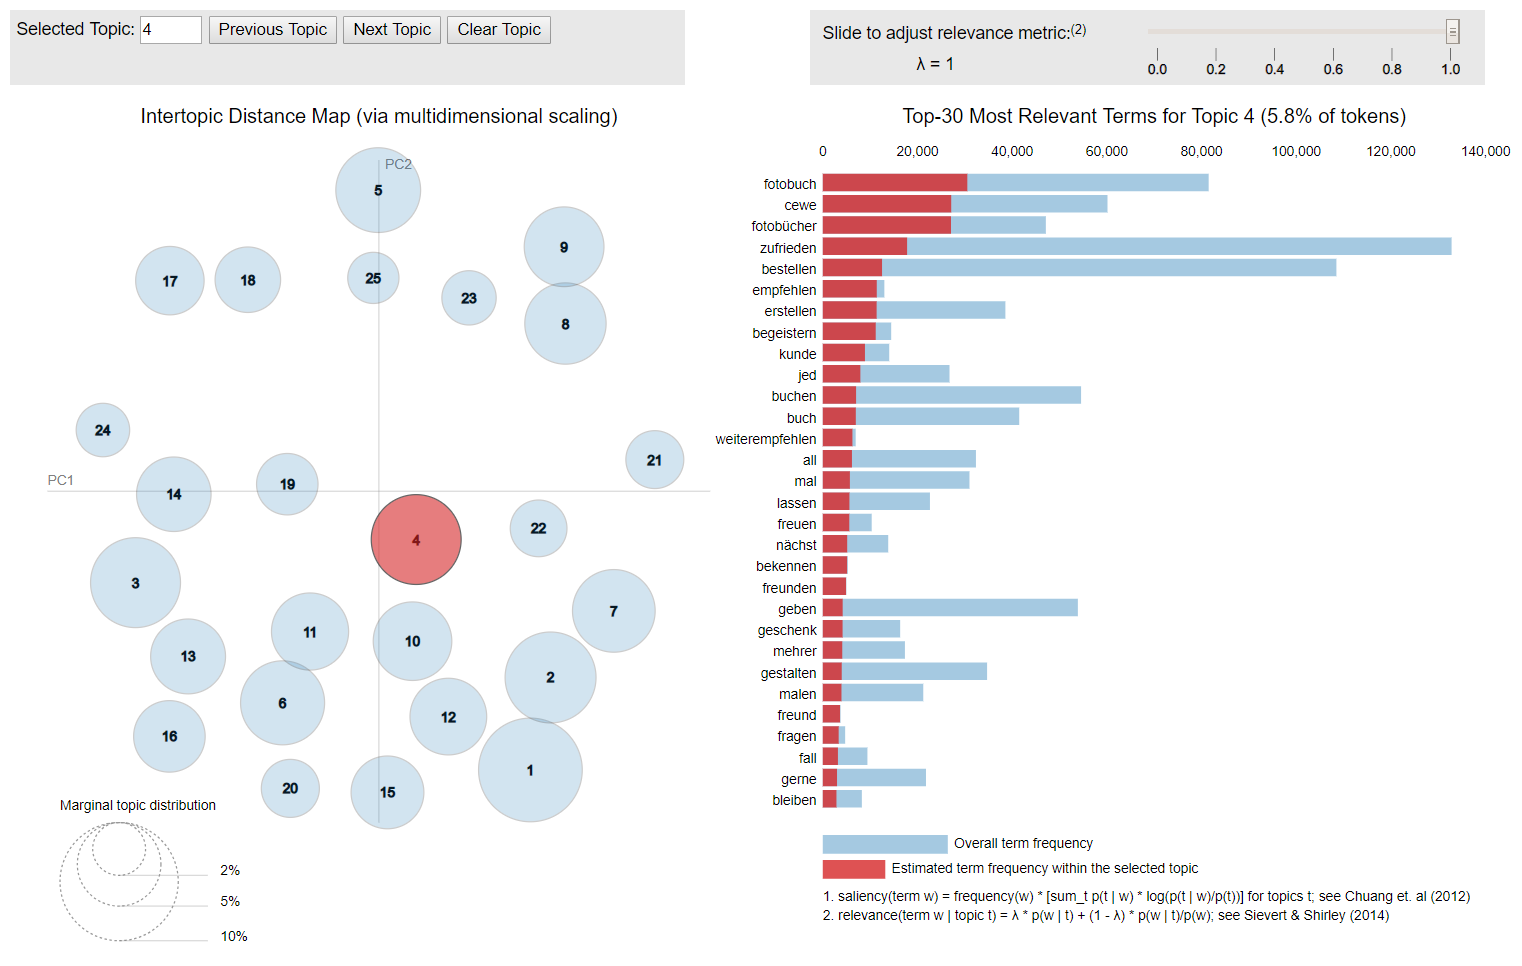
\includegraphics[scale=0.65, angle=-90]{vis_result.png}
        \end{center}
        \caption{Screenshot of the Modelling Visualization}
    \end{figure}
    \newpage
    \section{Summary}

    \section{Outlook}
    Generalize the system, provide an interfaces where get different parsers.

    The evaluation metrics and be improved. Some results from different topic coherence indexes conflict with each other. For example, topic coherence generated from c\textunderscore{}umass \cite{mimno_optimizing_nodate} and c\textunderscore{}v \cite{roder_exploring_2015} are often negatively correlated.

    Better user interface, utilizing tools such as Semantic UI.

    Containerize the system.

    % Configure distributed version

    \section*{Acknowledgments}

    \bibliographystyle{IEEEtran}
    \bibliography{Library, gensim}

\end{document}
